\documentclass{beamer}
%
% Choose how your presentation looks.
%
% For more themes, color themes and font themes, see:
% http://deic.uab.es/~iblanes/beamer_gallery/index_by_theme.html
%
\mode<presentation>
{
  \usetheme{default}      % or try Darmstadt, Madrid, Warsaw, ...
  \usecolortheme{default} % or try albatross, beaver, crane, ...
  \usefonttheme{default}  % or try serif, structurebold, ...
  \setbeamertemplate{navigation symbols}{}
  \setbeamertemplate{caption}[numbered]
  \setbeamertemplate{footline}[frame number]
} 

\usepackage[english]{babel}
\usepackage[utf8x]{inputenc}
\usepackage{listings}
\usepackage{courier}
\usepackage{array}

\title[2016-05-11-scala-spark]{Scala and Spark Tutorial}
\author{Jim Pivarski}
\institute{Princeton University -- DIANA}
\date{May 11, 2016}

\xdefinecolor{darkblue}{rgb}{0.1,0.1,0.7}
\xdefinecolor{darkgrey}{rgb}{0.35,0.35,0.35}
\definecolor{commentgreen}{rgb}{0,0.6,0}
\definecolor{stringmauve}{rgb}{0.58,0,0.82}

\lstset{ %
  backgroundcolor=\color{white},      % choose the background color
  basicstyle=\ttfamily\scriptsize,         % size of fonts used for the code
  breaklines=true,                    % automatic line breaking only at whitespace
  captionpos=b,                       % sets the caption-position to bottom
  commentstyle=\color{commentgreen},  % comment style
  escapeinside={\%*}{*)},             % if you want to add LaTeX within your code
  keywordstyle=\color{blue},          % keyword style
  stringstyle=\color{stringmauve},    % string literal style
  showstringspaces=false,
  showlines=true
}

\lstdefinelanguage{scala}{
  morekeywords={abstract,case,catch,class,def,%
    do,else,extends,false,final,finally,%
    for,if,implicit,import,match,mixin,%
    new,null,object,override,package,%
    private,protected,requires,return,sealed,%
    super,this,throw,trait,true,try,%
    type,val,var,while,with,yield},
  otherkeywords={=>,<-,<\%,<:,>:,\#,@},
  sensitive=true,
  morecomment=[l]{//},
  morecomment=[n]{/*}{*/},
  morestring=[b]",
  morestring=[b]',
  morestring=[b]"""
}

\begin{document}

\begin{frame}
  \titlepage
\end{frame}

% Uncomment these lines for an automatically generated outline.
%\begin{frame}{Outline}
%  \tableofcontents
%\end{frame}

\begin{frame}{}
\begin{description}
\item[Spark:] a data analysis framework

(like ROOT, but with different strengths and weaknesses).

\vspace{0.5 cm}

\item[Scala:] Spark's native language, used as a command prompt

(the way that C++ is used for ROOT).
\end{description}
\end{frame}

\begin{frame}{Outline}
\begin{enumerate}
\item 5 minute talk on Scala
\item $\sim$half hour Scala exercises
\item 5 minute talk on Spark
\item $\sim$hour and a half Spark exercises in Scala
\end{enumerate}
\end{frame}

\begin{frame}{}
\begin{columns}
\column{1.1\linewidth}
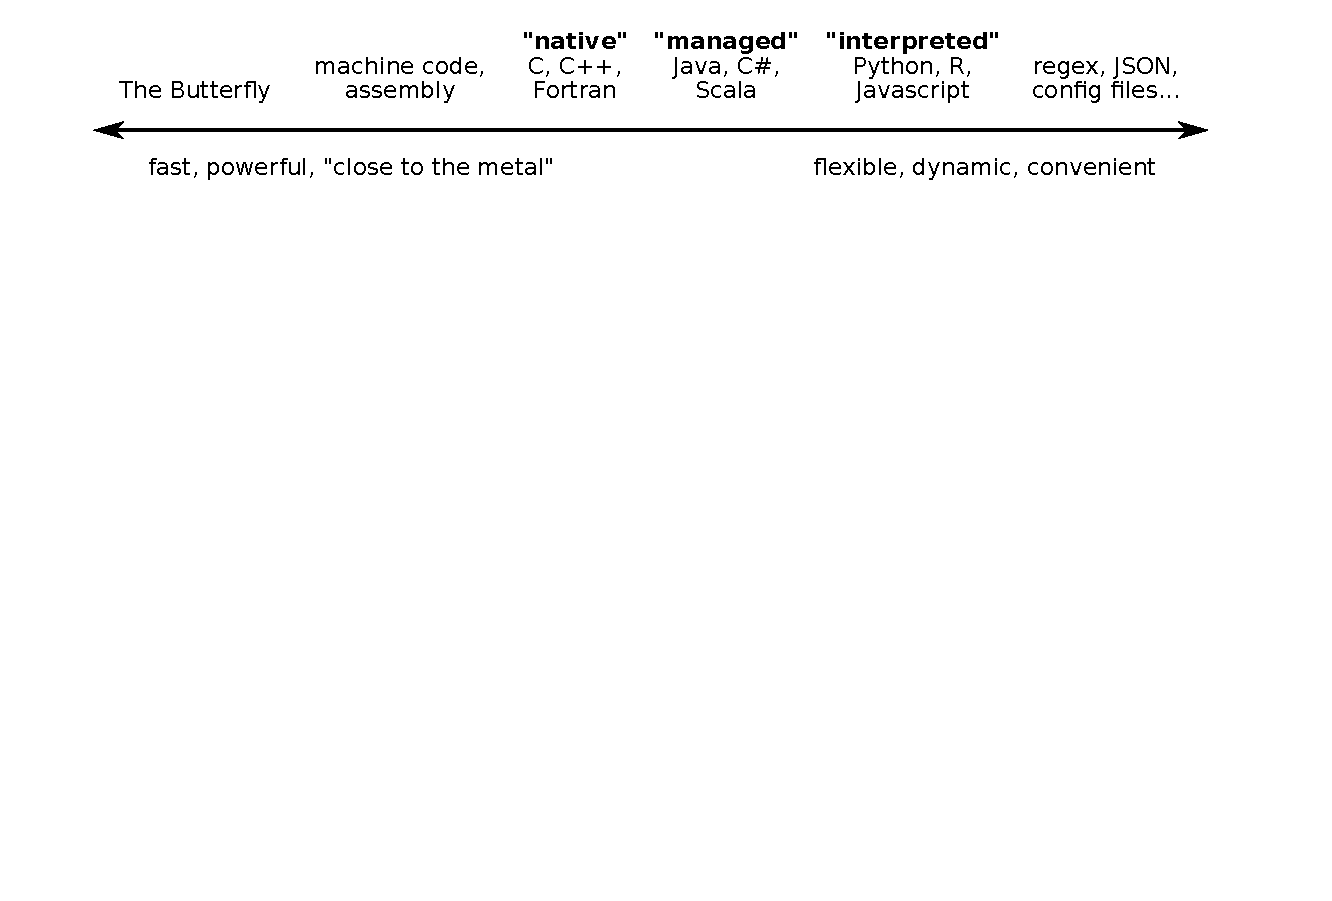
\includegraphics[width=\linewidth]{languages1.pdf}
\end{columns}
\end{frame}

\begin{frame}{}
\begin{columns}
\column{1.1\linewidth}
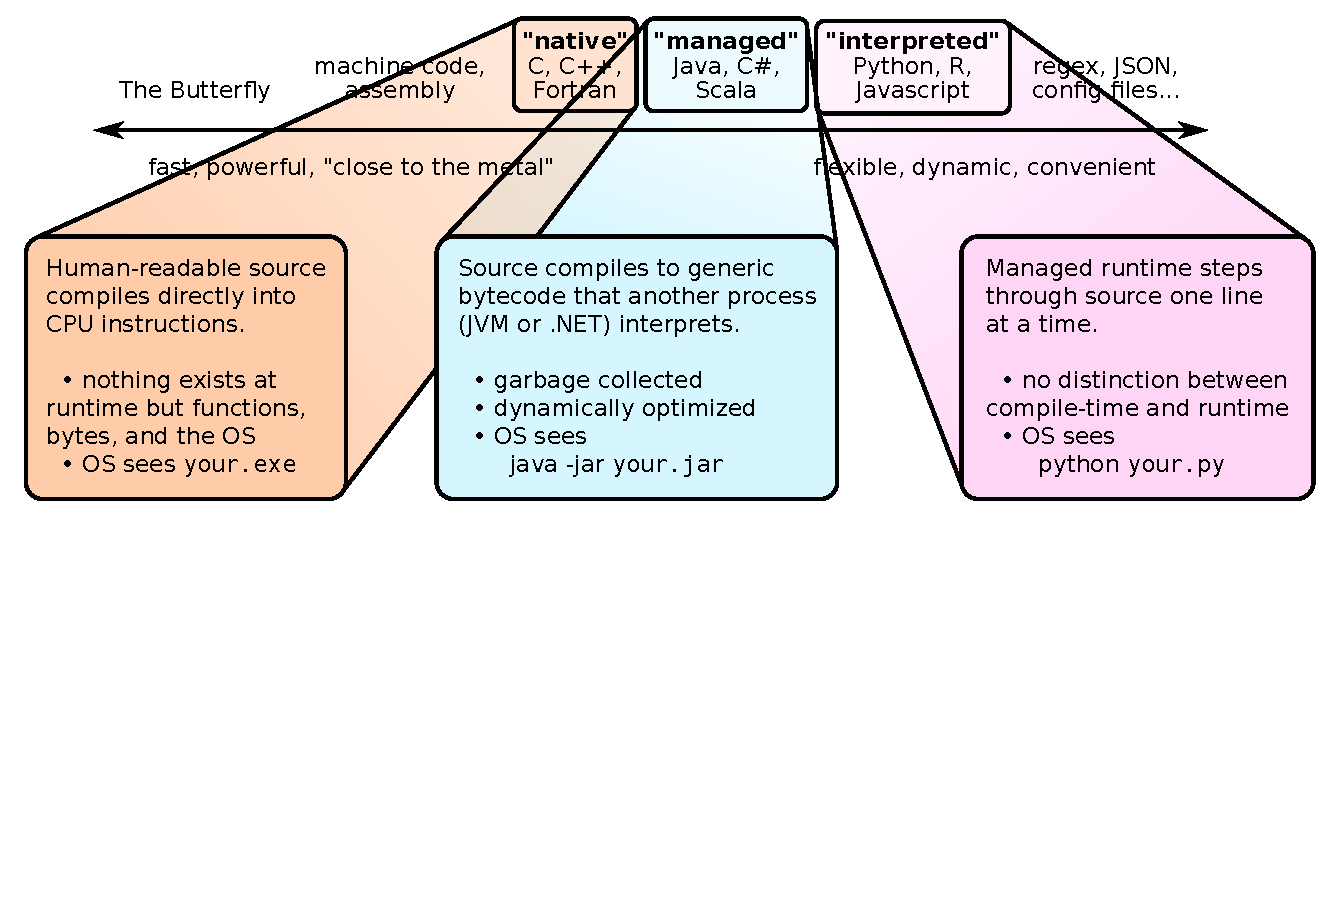
\includegraphics[width=\linewidth]{languages2.pdf}
\end{columns}
\end{frame}

\begin{frame}{}
\begin{columns}
\column{1.1\linewidth}
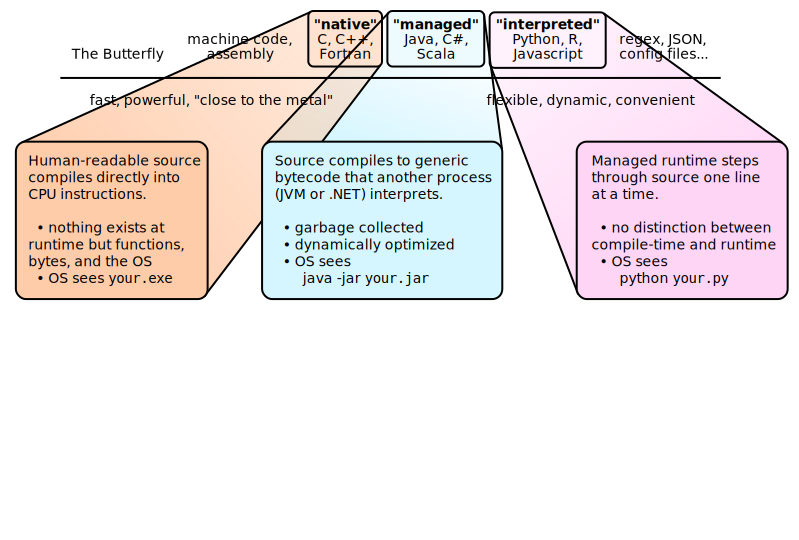
\includegraphics[width=\linewidth]{languages25.pdf}
\end{columns}
\end{frame}

\begin{frame}{}
\begin{center}
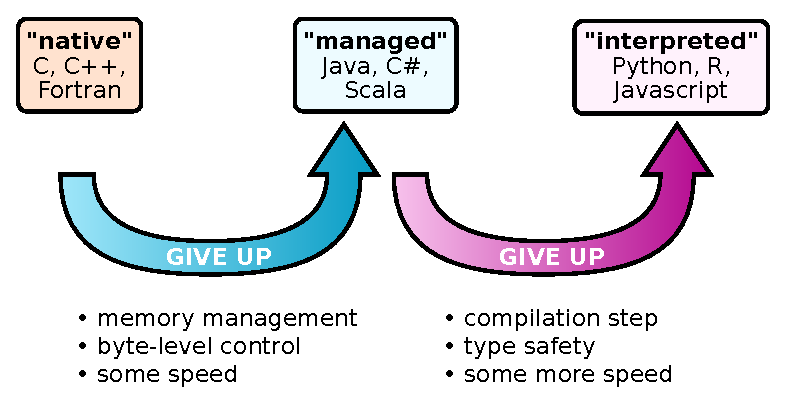
\includegraphics[width=0.8\linewidth]{languages3.pdf}
\end{center}
\end{frame}

\begin{frame}{}
\begin{center}
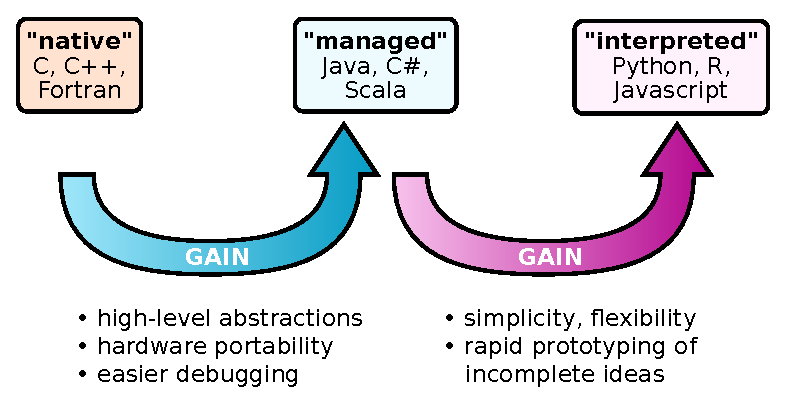
\includegraphics[width=0.8\linewidth]{languages4.pdf}
\end{center}
\end{frame}

\begin{frame}{What happens in the compilation step?}
\begin{itemize}
\item Whole program is interpreted and turned into machine instructions (possibly for a virtual machine).
\item All variables are interpreted as belonging to specific types: {\tt int}, {\tt string}, {\tt MissileController}\ldots
\item Uses of these variables are checked for validity:
\begin{itemize}
\item can't pass a {\tt MissileController} into the cosine function;
\item can't call {\tt launchAllMissiles()} on a {\tt string}.
\end{itemize}
\end{itemize}

\vfill
Interpreted languages do none of these things; you find out about misuses of variables at runtime (can be good, can be bad).
\end{frame}

\begin{frame}{Why should you care?}
\begin{itemize}
\item Compilation step can get in the way of testing a program one piece at a time.
\item The type check is a {\it formal proof} that the program is free of certain types of errors; it won't fail after hours of running.
\end{itemize}

\vfill
\begin{uncoverenv}<2->
\hspace{-0.83 cm} \textcolor{darkblue}{\Large Scala}

\begin{itemize}
\item Scala compiles to bytecode that runs on the Java Virtual Machine (JVM).
\item It emphasizes type safety (even more than C++).
\item It has extensive type inference to reduce annoyance,
\item and an interactive prompt for testing small components or interacting with a running program.
\end{itemize}
\end{uncoverenv}
\end{frame}

\begin{frame}{}
\begin{columns}
\column{1.18\linewidth}
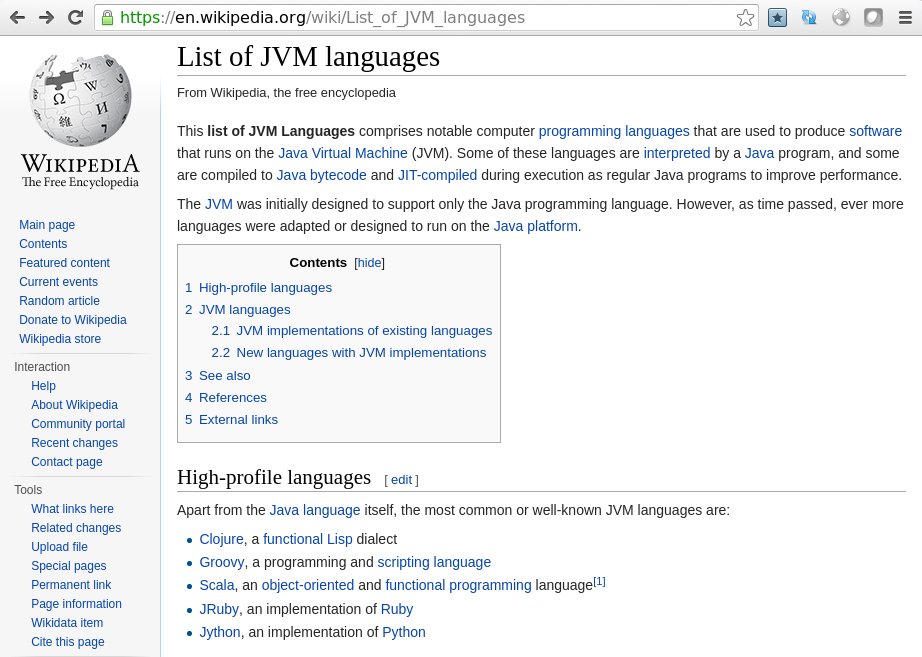
\includegraphics[width=\linewidth]{jvm_languages.png}
\end{columns}
\end{frame}

\begin{frame}{}
\begin{columns}
\column{1.18\linewidth}
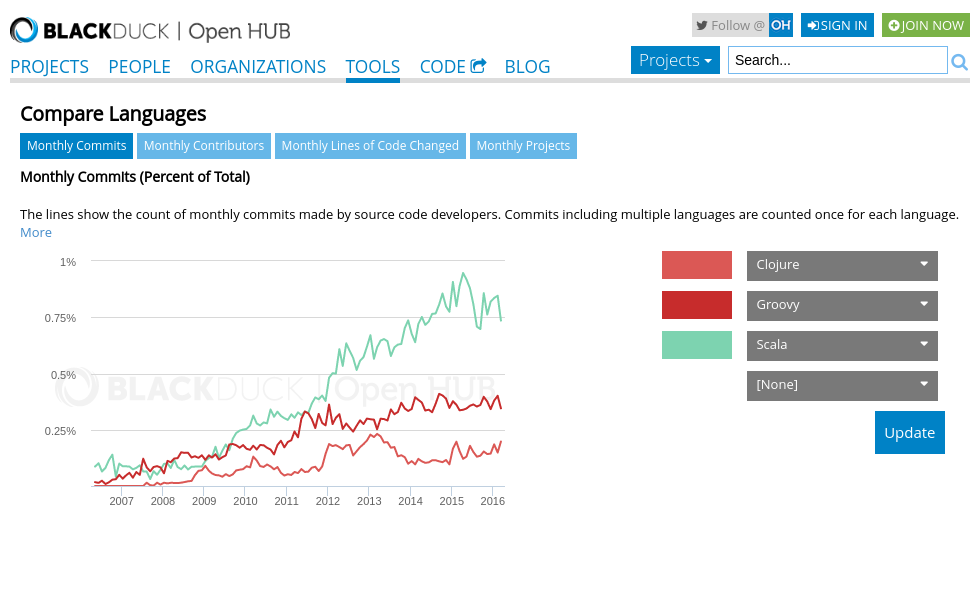
\includegraphics[width=\linewidth]{popularity1.png}
\end{columns}
\end{frame}

\begin{frame}{}
\begin{columns}
\column{1.18\linewidth}
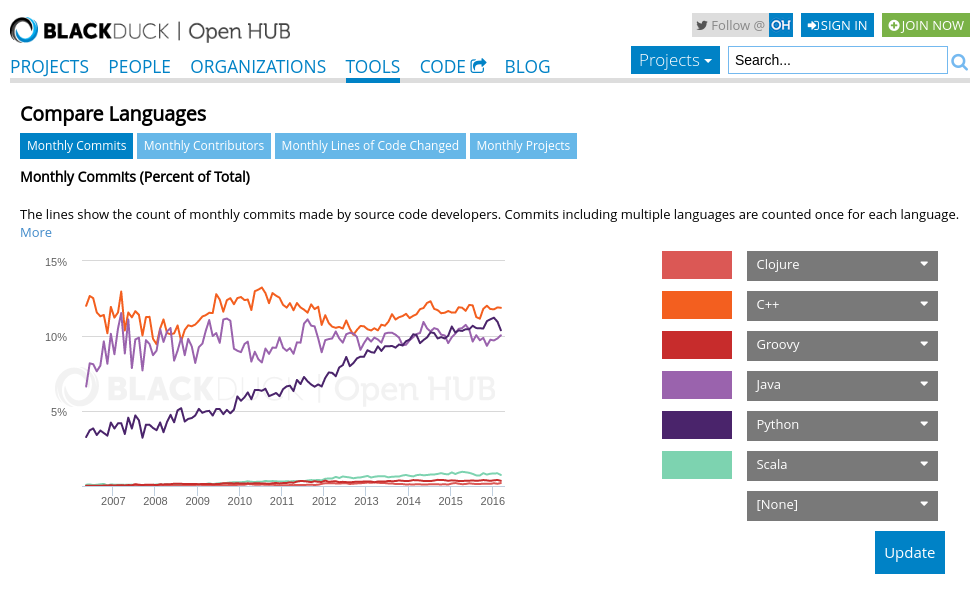
\includegraphics[width=\linewidth]{popularity2.png}
\end{columns}
\end{frame}

\begin{frame}{}
\begin{center}
\Huge \textcolor{darkblue}{Scala Exercises}
\end{center}
\end{frame}

{\usebackgroundtemplate{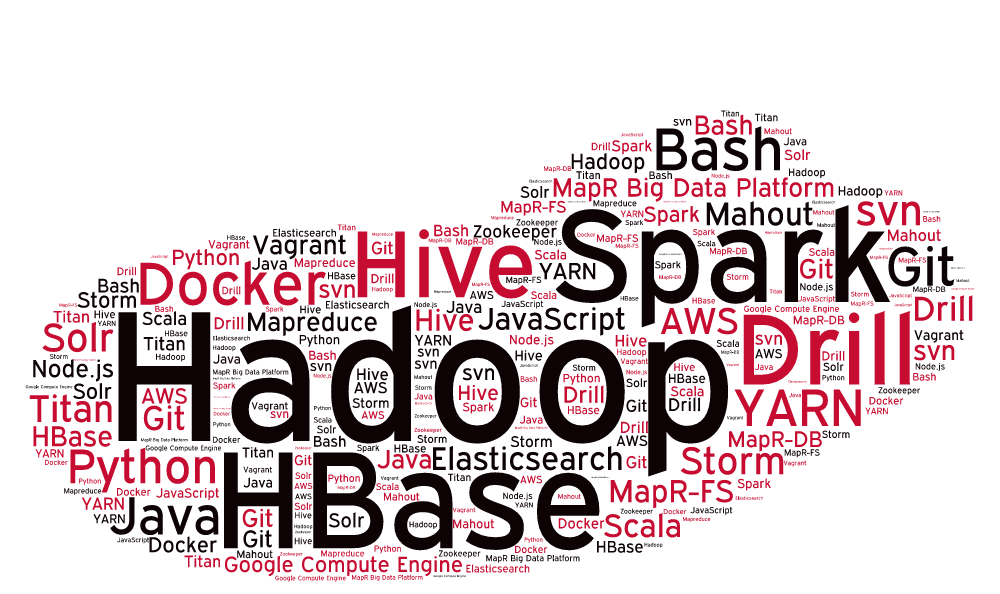
\includegraphics[width=\paperwidth]{word-cloud-07-2014_full.png}}
\begin{frame}{Big Data tools}
\end{frame}
}

{\usebackgroundtemplate{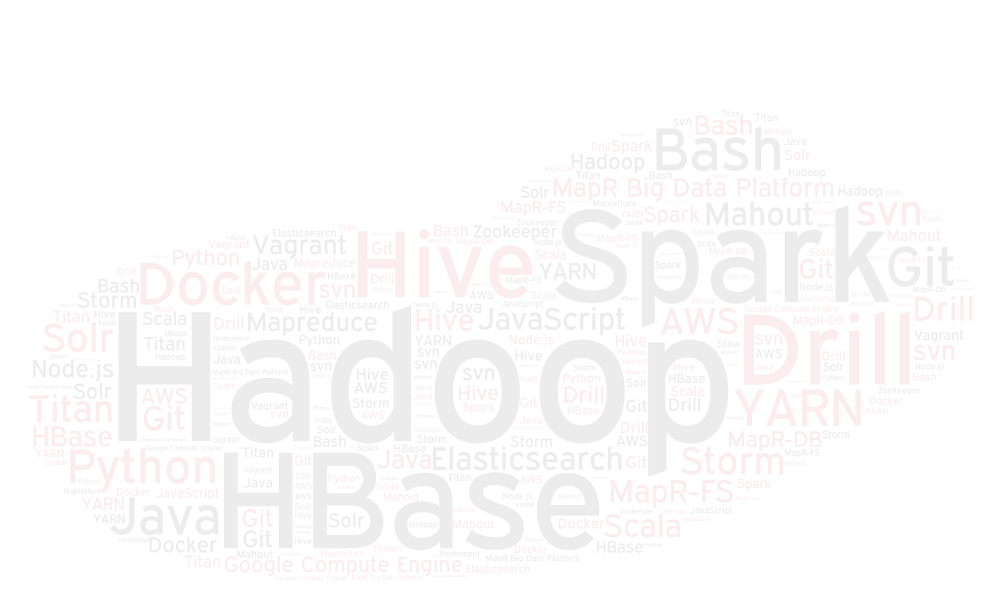
\includegraphics[width=\paperwidth]{word-cloud-07-2014.png}}
\begin{frame}{Big Data tools}
\begin{columns}
\column{0.4\linewidth}

\textcolor{darkblue}{Batch data analysis:}

\begin{itemize}
\item Apache Hadoop
\item {\only<1>{Apache Spark}\only<2>{\bf Apache Spark}}
\item Google TensorFlow
\end{itemize}

\textcolor{darkblue}{Query engines:}

\begin{itemize}
\item Elasticsearch
\item Apache Impala
\item Apache Drill
\item {\only<1>{Spark-SQL}\only<2>{\bf Spark-SQL}}
\end{itemize}

\textcolor{darkblue}{Data pipelines:}

\begin{itemize}
\item Apache Kafka
\item nsq
\end{itemize}

\column{0.4\linewidth}
\textcolor{darkblue}{Streaming data analysis:}

\begin{itemize}
\item Apache Storm
\item Apache Flink
\item {\only<1>{Spark-Streaming}\only<2>{\bf Spark-Streaming}}
\end{itemize}

\textcolor{darkblue}{Cluster infrastructures:}

\begin{itemize}
\item Apache HDFS
\item Apache Mesos
\end{itemize}

\textcolor{darkblue}{Machine learning:}

\begin{itemize}
\item Scikit-Learn
\item Apache Mahout
\item {\only<1>{Spark MLlib}\only<2>{\bf Spark MLlib}}
\end{itemize}
\end{columns}

\hfill \textcolor{blue}{\scriptsize \url{https://github.com/onurakpolat/awesome-bigdata}}
\end{frame}}

\begin{frame}{From Hadoop to Spark}
\vspace{-0.1 cm}
\begin{block}{2003--2004}
Google published {\it The Google File System} and {\it MapReduce: Simplified Data Processing on Large Clusters.}
\end{block}

\begin{block}{2006}
HDFS and Hadoop-MapReduce projects started at \\ Yahoo!\ but within Apache, fully open-source.

\vspace{-1.4 cm} \hfill 
\includegraphics[width=2 cm]{01_Hadoop_full.jpg}
\end{block}

\begin{block}{2008--2009}
Hadoop sorted TB--PB of data in record time. Started getting contributions from Facebook, LinkedIn, eBay, and IBM.
\end{block}

\begin{block}{2009}
Spark began as a class project at Berkley, targeting \\ {\it iterative} map-reduce for machine learning.

\vspace{-1.1 cm} \hfill 
\includegraphics[width=2 cm]{spark-logo.png}
\end{block}

\begin{block}{2013}
Spark became an Apache project and Databricks founded. In 2014, Spark won records for TB--PB sorting.
\end{block}
\end{frame}

\begin{frame}{Google Trends search results}
\begin{center}
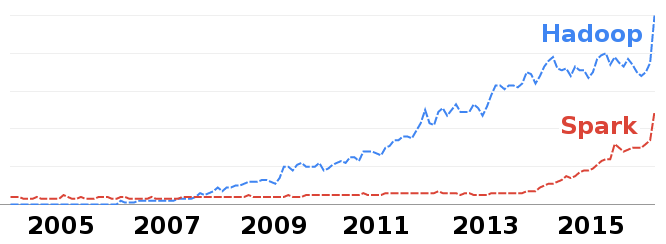
\includegraphics[width=0.9\linewidth]{trends.png}
\end{center}
\end{frame}

\begin{frame}{}
\begin{columns}
\column{0.65\linewidth}
Spark's specialty: caching data in RAM for iterative fits.

\vspace{0.2 cm}
Hadoop (and every other distributed batch system I've heard of) has to load data from disk for each pass.

\column{0.35\linewidth}
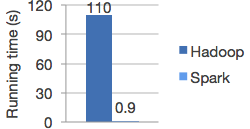
\includegraphics[width=\linewidth]{spark_time.png}
\end{columns}

\vfill
Beyond this killer app, Spark was designed for exploratory data analysis; Hadoop was designed for large applications.
\begin{itemize}
\item Native Spark runs on a command line in Scala (natively), Python, and R (through a bridge).
\item Hadoop asks the user to extend Mapper and Reducer classes.
\item Spark has many minor conveniences.
\item Spark generalizes on the map-reduce concept to chains of functional primitives.
\end{itemize}
\end{frame}

\begin{frame}[fragile]{Chains of functional primitives}

Functional programming style is common among data analysts using R (inherited from Scheme).

\vspace{0.2 cm}
Scala's object orientation lets us chain functors without nesting.

\vspace{0.2 cm}
\begin{columns}
\column{0.6\linewidth}
\begin{lstlisting}[language=c,frame=single]
for (i = 0;  i < nEvents;  i++) {
    event = events(i);
    if (condition(event))
        continue;
    add_to_output(calculation(event));
}
\end{lstlisting}
\column{0.42\linewidth}
\begin{lstlisting}[language=python,frame=single]

output =
  events.filter(condition)
        .map(calculation)


\end{lstlisting}
\end{columns}

\begin{itemize}
\item The ``map'' functor {\it says less} than ``for''--- it doesn't specify an order in which events must be processed.
\item Underlying system can distribute and collect however it likes.
\item Also hides index arithmetic from the user: datasets can be spliced automatically.
\end{itemize}
\end{frame}

\begin{frame}{``Monad-like'' functional primitives:}

Transforming one data table (ntuple) into another.

\vfill
\renewcommand{\arraystretch}{1.5}
\begin{tabular}{p{0.12\linewidth} >{\centering}p{0.08\linewidth} >{\centering}p{0.17\linewidth} >{\centering}p{0.08\linewidth} p{0.4\linewidth}}
& input & function & output & operation \\\hline
\textcolor{darkblue}{map} & table of $A$ & $f: A \to B$ & table of $B$ & apply $f$ to each row $A$, get a table of the same number of rows $B$ \\
& \multicolumn{4}{l}{\scriptsize \color{darkgrey} a.k.a. ``lapply'' (R), ``SELECT'' (SQL), list comprehension (Python)} \\
\textcolor{darkblue}{filter} & table of $A$ & $f: A \to \mbox{boolean}$ & table of $A$ & get a shorter table with the same type of rows \\
& \multicolumn{4}{l}{\scriptsize \color{darkgrey} a.k.a. single brackets (R), ``WHERE'' (SQL), list comprehension (Python)} \\
\textcolor{darkblue}{flatMap} & table of $A$ & $f: A \to \mbox{table of } B$ & table of $B$ & compose \textcolor{darkblue}{map} and \textcolor{darkblue}{flatten}, get a table of any length \\
& \multicolumn{4}{l}{\scriptsize \color{darkgrey} a.k.a. ``map'' (Hadoop), ``EXPLODE'' (SQL), $>>=$ (Haskell)} \\
\end{tabular}
\end{frame}

\begin{frame}{``Monoid-like'' functional primitives:}

Summarizing an ntuple using a counter, summation, or histogram.

\vfill
\renewcommand{\arraystretch}{1.5}
\begin{tabular}{p{0.12\linewidth} >{\centering}p{0.2\linewidth} >{\centering}p{0.23\linewidth} >{\centering}p{0.08\linewidth} >{\raggedright\arraybackslash}p{0.25\linewidth}}
& input & function(s) & output & operation \\\hline
\textcolor{darkblue}{reduce} & table of $A$ & $f: (A, A) \to A$ & single $A$ & apply $f$ to the running sum and one more element \\
\textcolor{darkblue}{aggregate} & table of $A$, initial value $B$ (``zero'') & $f: (A, B) \to B$ $f: (B, B) \to B$ (increment and combine) & single value $B$ & accumulate a counter with a different data type from the input \\
\textcolor{darkblue}{aggregate by key} & table of $\langle K,A \rangle$, initial value $B$ & $f: (A, B) \to B$ $f: (B, B) \to B$ & pairs $\langle K,B \rangle$ & aggregate independently for each key \\
& \multicolumn{4}{l}{\scriptsize \color{darkgrey} a.k.a. ``reduce'' (Hadoop), ``GROUP BY'' (SQL)} \\
\end{tabular}
\end{frame}

\begin{frame}{Associativity is key}

``Monad'' and ``monoid'' refer to mathematical properties of the operator, the most important being associativity, which allows the user's function to be dispatched arbitrarily.

\begin{center}
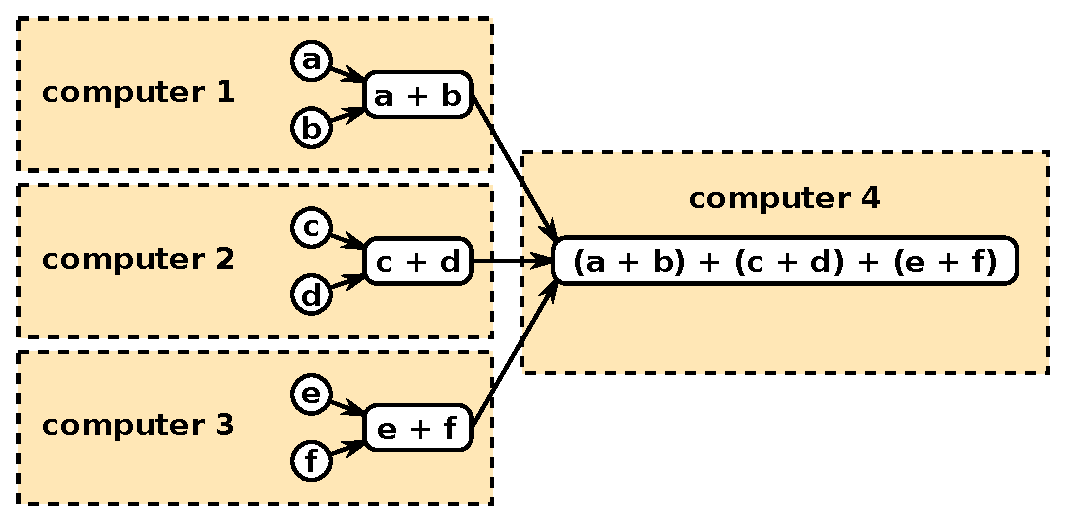
\includegraphics[width=0.7\linewidth]{monoids.pdf}
\end{center}
\end{frame}








\begin{frame}{}
\begin{center}
\Huge \textcolor{darkblue}{Spark Exercises}
\end{center}
\end{frame}

\end{document}
